\documentclass{article}
\usepackage[utf8]{inputenc}
\usepackage{amsmath, amssymb, multicol, enumerate, tikz}
\usepackage[margin = 0.5in]{geometry}
\pagestyle{empty}
\raggedright
\newcounter{PS}
\begin{document}

Name \makebox[3in]{\hrulefill} \hfill Honors Algebra 2 PSet

\subsubsection*{Absolute Value Equations and Inequalities \hfill \makebox[0.35in]{\hrulefill} / 10}

Solve each.
\begin{flalign*}
1.  \quad   &   |x-2| = 7   &
2.  \quad   &   |2x-3| = 11 &
3.  \quad   &   |x| = -3    &&\\[2.5in]
4.  \quad   &   2|y-1|=8    &
5.  \quad   &   |3x-1|+20=25    &
6.  \quad   &   |5x-8|=|3x+2|   &&\\
\end{flalign*}

\newpage

Name \makebox[3in]{\hrulefill} \hfill Hon. Alg. 2

\subsection*{Absolute Value Inequalities}

Solve each and graph your solution on a number line.
\begin{flalign*}
7.  \quad   &   |x-2|<1 &
8.  \quad   &   |2x-6|\leq 8    &
9.  \quad   &   |x-4| \geq 2    &&\\[2in]
10. \quad   &   |3x-8|>7    &
11. \quad   &   |x-2| < -1  &
12. \quad   &   |x+6| > -5  &&\\[2in]
\end{flalign*}

\subsection*{Challenge Problems}

Solve each of the following compound absolute value inequalities and graph your solution on a number line.
\begin{flalign*}
13. \quad   &   1 \leq |x-2| \leq 3 &
14. \quad   &   1 \leq |2x+1| < 3   &
15. \quad   &   0 < |2-x| \leq 2    &&\\[1.5in]
\end{flalign*}

Solve for $x$ in terms of the other variables. Assume $a$, $b$, and $c$ are positive numbers.
\begin{flalign*}
16. \quad   &   |x - a| \geq c  &
17. \quad   &   |a + bx| < c    &
18. \quad   &   b|x+a| > c  &&\\
\end{flalign*}

\newpage

\subsection*{Absolute Value Equations and Inequalities Answers}    \vspace{0.25in}

\begin{flalign*}
1.  \quad   &   x=-5 \text{ or } x = 9   &
2.  \quad   &   x=-4 \text{ or } x = 7   &
3.  \quad   &   \text{No Solution} (\varnothing)   &&\\
4.  \quad   &   y=-3 \text{ or } y=5 &
5.  \quad   &   x=-\frac{4}{3} \text{ or } x = 2   &
6.  \quad   &   x=\frac{3}{4} \text{ or } x =5    &&\\
\end{flalign*}


\begin{tabular}{p{0.3\textwidth}p{0.3\textwidth}p{0.3\textwidth}}
    7. $1 < x < 3$  &
    8. $-1 \leq x \leq 7$   &
    9. $x \leq 2$ or $x \geq 6$ \\[11pt]
    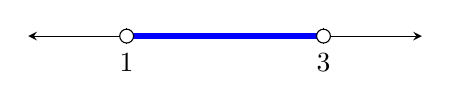
\begin{tikzpicture}
    \draw [<->, >=stealth] (-2.5,0) -- (2.5,0);
    \draw (-1.25,0.1) -- (-1.25,-0.1);
    \draw (1.25,0.1) -- (1.25,-0.1);
    \node at (-1.25,-0.1) [anchor=north] {$1$};
    \node at (1.25,-0.1) [anchor=north] {$3$};
    \draw [color=blue, line width=2] (-1.25,0)--(1.25,0);
    \draw [fill=white] (-1.25,0) circle (2.5pt);
    \draw [fill=white] (1.25,0) circle (2.5pt);
    \end{tikzpicture}
    &
    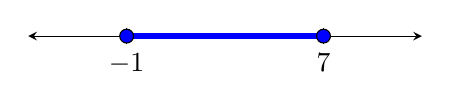
\begin{tikzpicture}
    \draw [<->, >=stealth] (-2.5,0) -- (2.5,0);
    \draw (-1.25,0.1) -- (-1.25,-0.1);
    \draw (1.25,0.1) -- (1.25,-0.1);
    \node at (-1.25,-0.1) [anchor=north] {$-1$};
    \node at (1.25,-0.1) [anchor=north] {$7$};
    \draw [color=blue, line width=2] (-1.25,0)--(1.25,0);
    \draw [fill=blue] (-1.25,0) circle (2.5pt);
    \draw [fill=blue] (1.25,0) circle (2.5pt);
    \end{tikzpicture}
    &
    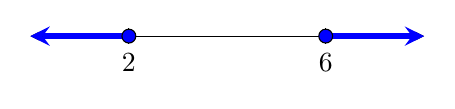
\begin{tikzpicture}
    \draw [<->, >=stealth] (-2.5,0) -- (2.5,0);
    \draw (-1.25,0.1) -- (-1.25,-0.1);
    \draw (1.25,0.1) -- (1.25,-0.1);
    \node at (-1.25,-0.1) [anchor=north] {$2$};
    \node at (1.25,-0.1) [anchor=north] {$6$};
    \draw [->, >=stealth, color=blue, line width=2] (-1.25,0)--(-2.5,0);
    \draw [->, >=stealth, color=blue, line width=2] (1.25,0)--(2.5,0);
    \draw [fill=blue] (-1.25,0) circle (2.5pt);
    \draw [fill=blue] (1.25,0) circle (2.5pt);
    \end{tikzpicture}
    \\[11pt]
    10. $x<\frac{1}{3}$ or $x>5$
    &
    11. No Solution $(\varnothing)$
    &
    12. All Real Numbers $(\mathbb{R})$
    \\[11pt]
    \raisebox{-0.75cm}{
    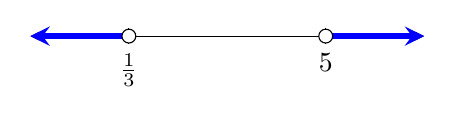
\begin{tikzpicture}
    \draw [<->, >=stealth] (-2.5,0) -- (2.5,0);
    \draw (-1.25,0.1) -- (-1.25,-0.1);
    \draw (1.25,0.1) -- (1.25,-0.1);
    \node at (-1.25,-0.1) [anchor=north] {$\frac{1}{3}$};
    \node at (1.25,-0.1) [anchor=north] {$5$};
    \draw [->, >=stealth, color=blue, line width=2] (-1.25,0)--(-2.5,0);
    \draw [->, >=stealth, color=blue, line width=2] (1.25,0)--(2.5,0);
    \draw [fill=white] (-1.25,0) circle (2.5pt);
    \draw [fill=white] (1.25,0) circle (2.5pt);
    \end{tikzpicture} }
    &
    \begin{tikzpicture}
    \draw [<->, >=stealth] (-2.5,0) -- (2.5,0);
    \draw (0,0.1) -- (0,-0.1);
    \end{tikzpicture}
    &
    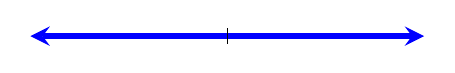
\begin{tikzpicture}
    \draw [<->, >=stealth, color=blue, line width = 2] (-2.5,0) -- (2.5,0);
    \draw (0,0.1) -- (0,-0.1);
    \end{tikzpicture}   \\
\end{tabular}

\end{document}
